\section{FrBu II.2 4}

\questionBox{
Sketch the following curve $\gamma$ ("figure eight")

%\[
%    \alfa(t)=\left\{
%    \begin{array}{lll}
%        1 - e^{it} & \text{for } t \in [0,2\pi]\\
%        -1 + e^{-it} & \text{for } t \in [2\pi, 4\pi].
%    \end{array}
%    \right.
%\]

\[
    \gamma(t)=\left\{
    \begin{array}{lll}
        1 - e^{i t} & \text{for } t \in [0,2 \pi]\\
        -1 + e^{-i t} & \text{for } t \in [2 \pi, 4 \pi].
    \end{array}
    \right.
\]

}

\answerBox{
Sketch of $\gamma$:

\begin{figure}[H]
    \centering
    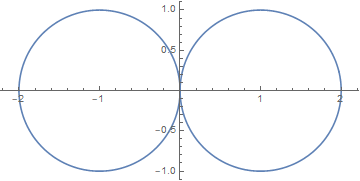
\includegraphics[width=0.5\textwidth]{pics/frbu214.png}
    %   \caption{}
\end{figure}
}